\documentclass{standalone}
\usepackage{color}
\usepackage{tikz}
\usepackage{pgfplots}
\usepackage{pgf-umlsd}
\usepackage{tikz}
\usetikzlibrary{positioning,calc}
\pgfplotsset{compat=1.16} 

%%%%%%%%
%Figure from: Rashid, Tabish, Mikayel Samvelyan, Christian Schroeder, Gregory Farquhar, Jakob Foerster, and Shimon Whiteson. "QMIX: Monotonic Value Function Factorisation for Deep Multi-Agent Reinforcement Learning." In International Conference on Machine Learning, pp. 4295-4304. 2018.
%%%%%%%%

\begin{document}
\pagestyle{empty}

\def\layersep{2.5cm}

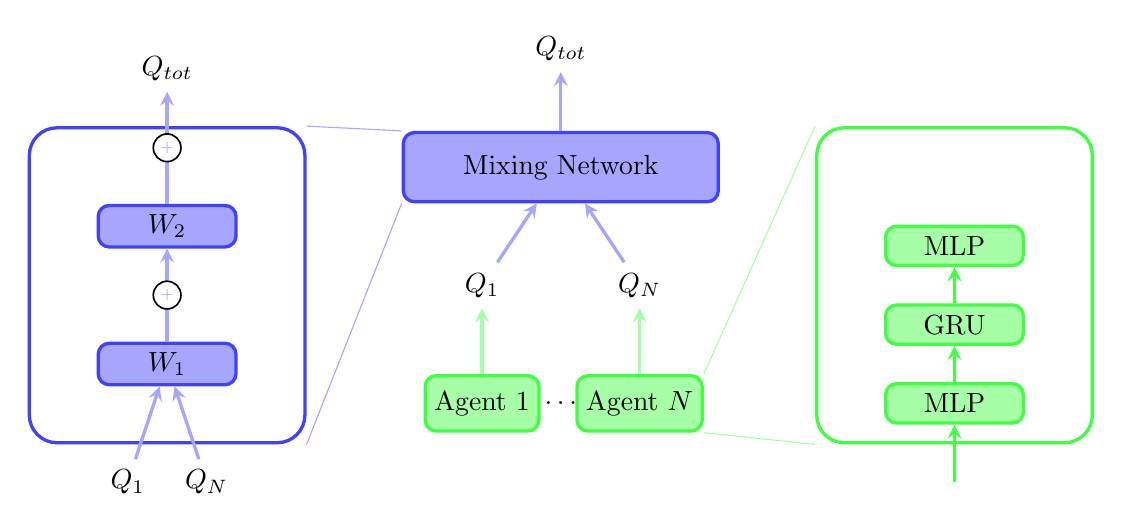
\begin{tikzpicture}[very thick]



\path (-1, 2) node[draw=green!75, fill=green!35, shape=rectangle, rounded corners, minimum height=20pt, minimum width=40pt] (agent1) {Agent $1$};
\path (1, 2) node[draw=green!75, fill=green!35, shape=rectangle, rounded corners, minimum height=20pt, minimum width=40pt] (agentn) {Agent $N$};
\path (0, 2) node (dots1) {$\dots$};

\path (0, 5) node[draw=blue!75, fill=blue!35, shape=rectangle, rounded corners, minimum height=25pt, minimum width=4cm] (mix) {Mixing Network};

\path (-1, 3.5) node (q1) {$Q_{1}$};
\path (1, 3.5) node (qn) {$Q_{N}$};
\path (0, 6.5) node (qtot) {$Q_{tot}$};

\draw[-stealth, green!35] (agent1) -- (q1);
\draw[-stealth, green!35] (agentn) -- (qn);
\draw[-stealth, blue!35] (q1) -- (mix);
\draw[-stealth, blue!35] (qn) -- (mix);
\draw[-stealth, blue!35] (mix) -- (qtot);

\path (-5, 3.5) node[draw=blue!75, shape=rectangle, rounded corners=10pt, minimum height=4cm, minimum width=3.5cm] (left) {
};
\path (5, 3.5) node[draw=green!75, shape=rectangle, rounded corners=10pt, minimum height=4cm, minimum width=3.5cm] (right) {
};

\path (-5, 2.5) node[draw=blue!75, fill=blue!35, shape=rectangle, rounded corners, minimum height=0.5cm, minimum width=1.75cm] (w1) {$W_{1}$
};
\path (-5, 4.25) node[draw=blue!75, fill=blue!35, shape=rectangle, rounded corners, minimum height=0.5cm, minimum width=1.75cm] (w2) {$W_{2}$
};
\draw[-stealth, blue!35] (w1) --node[draw=black, semithick, fill=white, minimum size= 10pt, inner sep=0, circle] {\tiny{+}} (w2);
\path (-5, 6.25) node (qtot1) {$Q_{tot}$};
\draw[-stealth, blue!35] (w2) --node[draw=black, semithick, fill=white, minimum size= 10pt, inner sep=0, circle] {\tiny{+}} (qtot1);
\draw[thin, blue!35] (mix.north west) -- (left.north east);
\draw[thin, blue!35] (mix.south west) -- (left.south east);
\draw[thin, green!35] (agentn.north east) -- (right.north west);
\draw[thin, green!35] (agentn.south east) -- (right.south west);
\path (-5.5, 1) node (q11) {$Q_{1}$};
\path (-4.5, 1) node (qn1) {$Q_{N}$};
\draw[-stealth, blue!35] (q11) -- (w1);
\draw[-stealth, blue!35] (qn1) -- (w1);

\path (5, 2) node[draw=green!75, fill=green!35, shape=rectangle, rounded corners, minimum height=0.5cm, minimum width=1.75cm] (mlp1) {MLP};
\path (5, 3) node[draw=green!75, fill=green!35, shape=rectangle, rounded corners, minimum height=0.5cm, minimum width=1.75cm] (gru) {GRU};
\path (5, 4) node[draw=green!75, fill=green!35, shape=rectangle, rounded corners, minimum height=0.5cm, minimum width=1.75cm] (mlp2) {MLP};
\draw[-stealth, green!75] (5, 1) -- (mlp1);
\draw[-stealth, green!75] (mlp1) -- (gru);
\draw[-stealth, green!75] (gru) -- (mlp2);
\end{tikzpicture}
% End of code
\end{document}